\chapter{Калибровка атомно-зондового томографа ПАЗЛ-3D}\label{ch:ch3}

\section{Верификация точности восстановления координат}\label{sec:ch3/sect1}

Определение пространственного разрешения атомно-зондового томографа обычно проводится при исследовании чистого металла с последующим анализом наличия/отсутствия атомных плоскостей. В случае, если пространственное разрешение установки равно или меньше чем расстояние между атомными плоскостями, разрешение установки считается равным или меньше чем расстояние атомными плоскостями, отвечающими тому или иному кристаллографическому направлению. Для верификации точности восстановления 3D координат был выбран поликристаллический вольфрам  \cite{scbibAPPLE}. Данный материал имеет ряд преимуществ для калибровочных процедур, таких как: отсутствие оксидного слоя, высокую температуру плавления, простоту изготовления образцов и кубическую объемно-центрированную решетку с параметром решетки 0.316 нм. Для подтверждения характеристик используется не менее 3 успешных исследований материала. Условия проведения исследования: температура образцов 22 К, частота работы лазера 25 кГц, мощность лазерного излучения не более 20 мВт, длина волны лазерного излучения 515 нм, скорость сбора данных от 60 до 250 событий/секунду. Пример полученного масс-спектра показан на рисунке \cref{fig:W_massspectr}. На масс-спектре отчетливо различимы пики всех стабильных изотопов вольфрама. Наблюдаемая зарядность ионов составила 3+. 

\begin{figure}[htb]
	\centerfloat{
		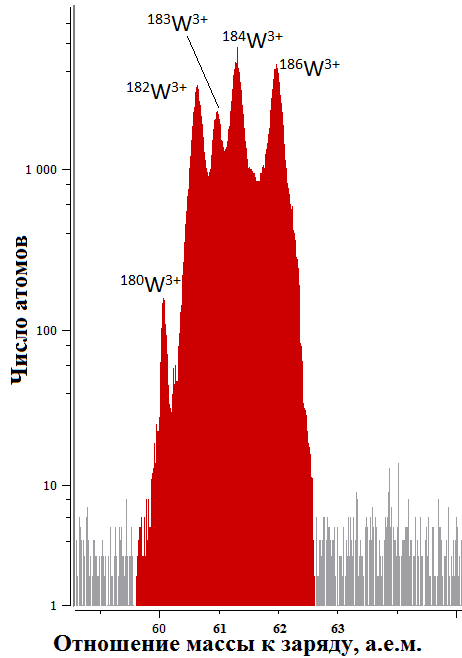
\includegraphics[width=.5\textwidth]{W_massspectr}
	}
	\caption{Масс-спектр образца из вольфрама}
	\label{fig:W_massspectr}
\end{figure}

Для оценки расстояния между атомными плоскостями были взяты отдельные части 3D объема в местах выхода кристаллографических направлений. Области выхода кристаллографических направлений определялись по двумерной гистограмме распределения событий на детектирующей системе, собранных за некоторый промежуток времени (Рисунок \cref{fig:W_3D}).

\begin{figure}[htb]
	\centerfloat{
		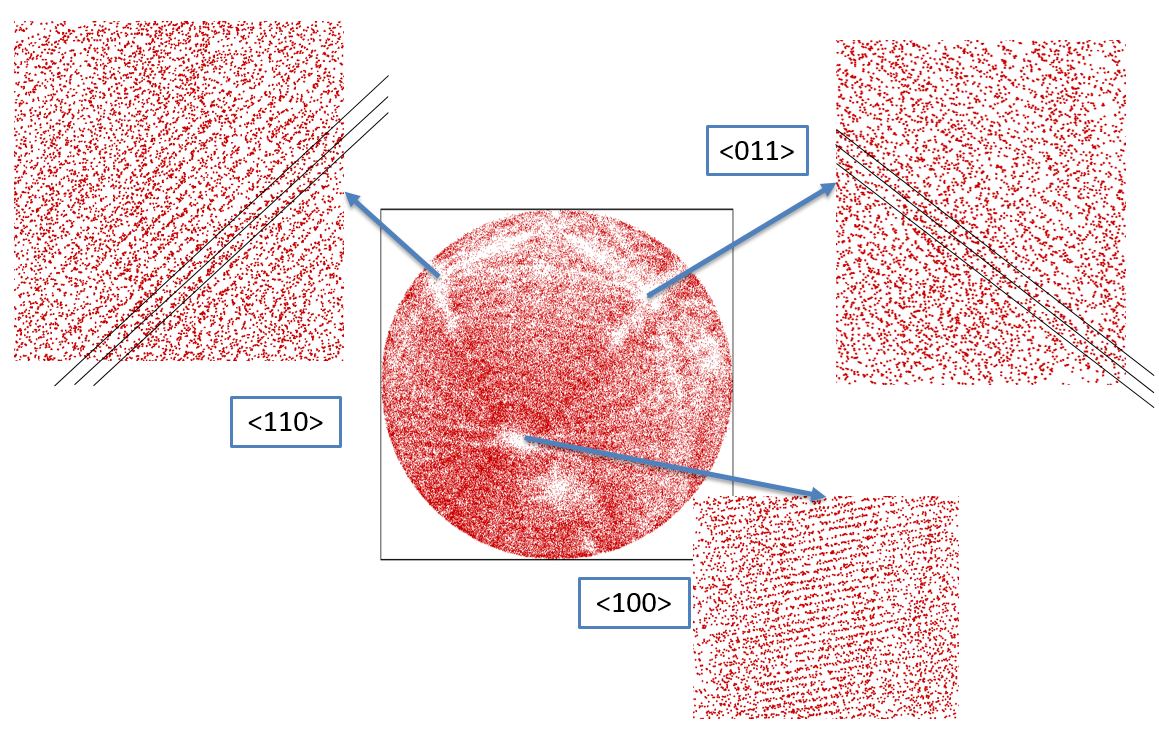
\includegraphics[width=\textwidth]{W_3D}
	}
	\caption{2D гистограмма распределения задетектированных событий}
	\label{fig:W_3D}
\end{figure}

Для каждого набора атомных плоскостей было определено среднее межплоскостное расстояние. Для выхода направления (100) измеренное расстояние составило 1.58 $\pm$ 0.03 \r{А}, что совпадает с табличным значение для вольфрама 1.58 \r{A} в переделах погрешности. Поскольку в данных исследованиях выход (100) ориентирован вдоль оси образца, то способность установки наблюдать атомные плоскости позволяет оценить разрешающую способность прибора вдоль оси образца (Z) в не более чем 1-2 \r{A}. Для выходов (011) также было измерено межплоскостное расстояние: 1.9 $\pm$ 0.3 \r{A}, что также согласуется с табличным значением в 2.2 \r{A}. Наборы плоскостей (011) и (110) расположены под углом к оси образца, это позволяет оценить латеральное разрешение установки: 2-4 \r{A}. Полученные оценки разрешающей способности ПАЗЛ-3D  характерны для большинства атомно-зондовых томографов. 

\FloatBarrier

\section{Первичная оценка оптимальных значений параметров лазерного испарения}\label{sec:ch3/sect2}

Для проведения первых исследований необходимо определить перечень параметров исследования, которые необходимо подбирать для получения качественных данных. К наиболее простым и показательным параметрам точности восстановления данных можно отнести разрешение по массе и пространственное разрешение. На основе литературного обзора можно заключить, что разрешение по массе, в случае применения аналогичной длины волны лазера, главным образом будет зависеть от длины пролетного промежутка. Исходя из данных, приведенных в Таблице \cref{tab:calcFWHM}, можно заключить, что ожидаемое разрешение по массе на используемой установке лежит в пределах от 360 до 1140 на полувысоте основного пика в зависимости от массы иона и ускоряющего напряжения. Пространственное разрешение у аналогичных приборов составляет примерно 3 \r{A} в плоскости, параллельной детектору, и менее 1 \r{A} в перпендикулярной плоскости и будет характеризоваться видимостью атомных плоскостей вдоль кристаллографических направлений. Успешность в достижении этих параметров будет проверена на примере одной из доступных для отработки методики стали Fe-13.5Cr-0.3Ti.

Достижение вышеперечисленных параметров является первоначальной целью проводимой работы. Для получения этих «целевых» показателей, необходимо получить зависимости качества данных от более широкого ряда параметров. К варьируемым параметрам эксперимента относятся температура образца, мощность лазера и скорость сбора данных (поток событий). Также на качество данных будут влиять: форма образца, поляризация лазерного излучения на образце, длина волны лазера и частота работы лазера. Для первичного подбора выбраны следующие параметры исследования: мощность лазера и поляризация лазерного излучения.

В случае АЗТ с лазерным испарением, практически все параметры эксперимента с хорошей точностью могут быть непосредственно взяты по аналогии с описанными в литературе экспериментами.  Исключение составляет мощность лазера, которая необходима для активации процесса полевого испарения. Каждая модель прибора АЗТ имеет уникальную лазерную систему, систему заведения пучка в анализационный объем, вследствие чего различен сам диаметр пучка \cite{Tu15}. Для проведения первых экспериментов, необходимо приблизительно оценить мощность лазера, чтобы иметь представление о диапазоне, в котором проводить первые исследования.

Универсальной величиной, учитывающей мощность лазера в  импульсе, подводимой к образцу, и фокусировку пучка, является плотность потока энергии $\rho_{e}$ – энергия, приходящаяся на единицу площади за импульс. Именно эта величина указывается в большинстве статей как основная характеристика пучка, подводимого к исследуемому образцу. В случаях, когда указывается энергия пучка за импульс и диаметр пучка у образца, можно выполнить пересчет до плотности потока энергии:

\begin{equation}
	\label{eq:oleg1}
	\rho_{e} = \frac{E}{s}
\end{equation}

где $\rho_{e}$ - плотность энергии, $Е$ - энергия пучка за импульс, $s$ – площадь поперечного сечения пучка.

Набор необходимых значений $\rho_{e}$  можно получить из ряда работ, посвященных разработке подобных установок. В расчет будут приняты данные работ, в которых длительность импульса и длина волны примерно совпадают с теми, которые предполагается использовать в настоящей работе. В Таблице~\cref{tab:energy_laser} приведены  используемые на аналогичных установках плотности энергии с указанием используемой длины волны, длительности импульса и материала.

\begin{table} [htbp]
	\centering
	\caption{Технические характеристики АЗТ установок с лазерным испарением. Исследуемый материал - вольфрам}
	\label{tab:energy_laser}
	\begin{SingleSpace}
		\begin{tabular} {| c | c | c | c | c | c |}
			\hline
			\thead{Плотность энергии, мкДж/мм$^{2}$} & \thead{Длина волны лазера, нм} & \thead{Длительность\\импульса, фс} & \thead{Источник}  \\ \hline
			150 & 780 &  120 &   \cite{Gault06_femto}             \\ \hline
			160 & 780  &  120 &  \cite{Vurpillot06}   		  	  \\ \hline
			160 & 525  &  100 &  \cite{Cerezo06}             \\ \hline			
		\end{tabular}
	\end{SingleSpace}
\end{table}


Таким образом, необходимая плотность энергии составляет примерно 160 мкДж/мм$^{2}$. 
Однако непосредственное измерение плотности энергии на рассматриваемом стенде  невозможно. Имеющимися средствами возможно измерение только средней мощности пучка перед системой его заведения в анализационный объем (Рисунок~ \cref{fig:Oleg_laser_schema}).

\begin{figure}[htb]
	\centerfloat{
		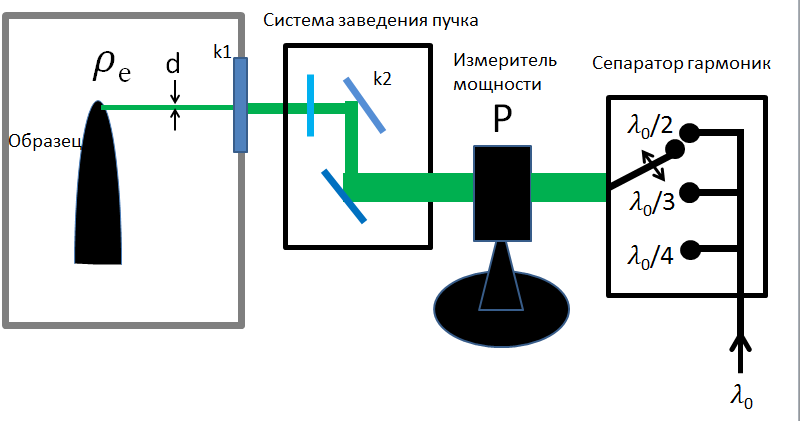
\includegraphics[width=\textwidth]{Oleg_laser_schema}
	}
	\caption{Схема контроля мощности лазера в используемой установке}
	\label{fig:Oleg_laser_schema}
\end{figure}

Зная необходимую плотность энергии $\rho_{e}$, диаметр пучка d, до которого проведена фокусировка и частоту работы лазера f, можно найти мощность P (Формула \cref{eq:oleg3}), непосредственно измеряемую измерителем мощности перед системой заведения пучка, учитывая коэффициент потерь k (см. формула \cref{eq:oleg2}).

\begin{equation}
	\label{eq:oleg2}
	k = k_{1} * k_{2},
\end{equation}

где $k_{1}$ - коэффициент потери мощности лазерного излучения при прохождении через окно анализационного объема, $k_{2}$ - коэффициент потери мощности лазерного излучения на зеркалах системы заведения.

\begin{equation}
	\label{eq:oleg3}
	P = \rho_{e}*\pi*\frac{d^{2}*f}{4*k}
\end{equation}

Таким образом, исходя из параметров установки ПАЗЛ (f = 50кГц, k = 0.4, d = 30 мкм), получаем:

\begin{equation}
	\label{eq:oleg4}
	P = 13 \pm 6 мВт
\end{equation}	

Следующим шагом является экспериментальный подбор мощности лазера. Мощность лазера (энергия импульса) является параметром, влияющим на ряд характеристик качества данных. Было проведено несколько экспериментов с различной мощностью на примере ДУО стали Fe-13.5Cr-0.3Ti. Рассмотрим эксперименты с мощностями 2 мВт, 10 мВт и 20 мВт. Масс-спектры приведены на Рисунках \cref{fig:Oleg_mass_spectr_2mv,fig:Oleg_mass_spectr_20mv,fig:Oleg_mass_spectr_10mv}. Во всех исследованиях температура образца составляла 50 К, частота работы лазера не менялась.

\begin{figure}[htb]
	\centerfloat{
		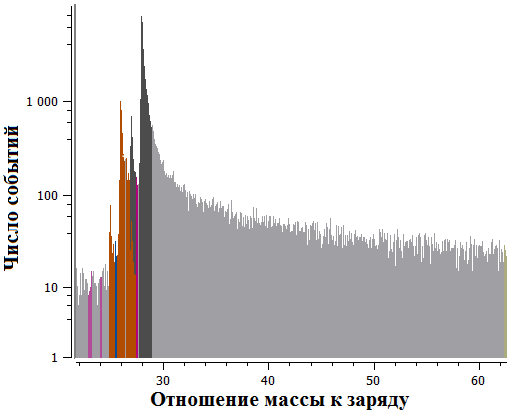
\includegraphics[width=.6\textwidth]{Oleg_mass_spectr_2mv}
	}
	\caption{Масс-спектр образца стали Fe-13.5Cr-0.3Ti при мощности 2 мВт}
	\label{fig:Oleg_mass_spectr_2mv}
\end{figure}

Как видно из Рисунка \cref{fig:Oleg_mass_spectr_2mv}, при столь низкой мощности (2 мВт), для достижения необходимого потока событий напряжение на образце было поднято до значений, при которых высока вероятность неконтролируемой ионизации атомов исследуемого образца. Это приводит к тому, что шум перекрывает все пики, стоящие правее железа (M/z $\sim$ 28), включая пики вольфрама (M/z $\sim$ 60). Высокий шум приводит к существенно большей сложности в определении малых значений концентраций элементов в образце.

\begin{figure}[htb]
	\centerfloat{
		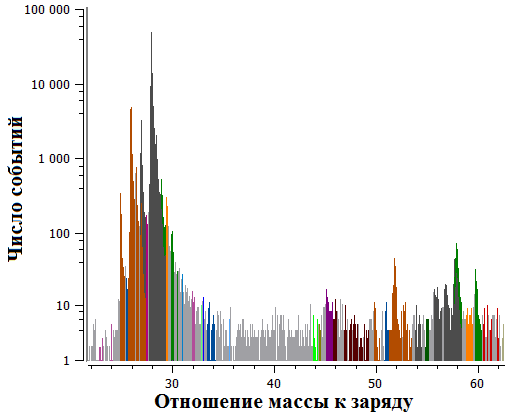
\includegraphics[width=.6\textwidth]{Oleg_mass_spectr_20mv}
	}
	\caption{Масс-спектр образца стали Fe-13.5Cr-0.3Ti при мощности 20 мВт}
	\label{fig:Oleg_mass_spectr_20mv}
\end{figure}

При мощности 20 мВт шум на масс-спектре минимален, но происходит испарение атомов с менее выгодной степенью ионизации (а также молекулярных ионов), что может приводить к нарушениям определения химического состава, а также затруднять расшифровку масс-спектра.

\begin{figure}[htb]
	\centerfloat{
		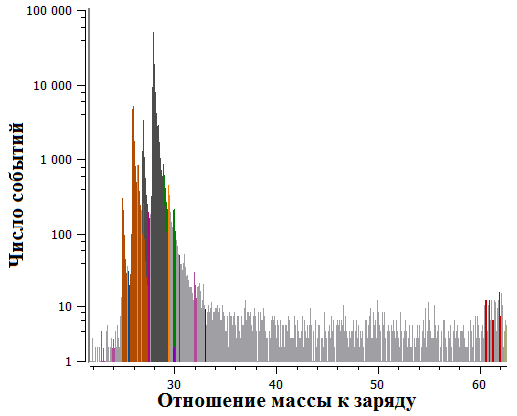
\includegraphics[width=.6\textwidth]{Oleg_mass_spectr_10mv}
	}
	\caption{Масс-спектр образца стали Fe-13.5Cr-0.3Ti при мощности 10 мВт}
	\label{fig:Oleg_mass_spectr_10mv}
\end{figure}

При мощности 10 мВт проведение исследований выглядит наиболее оптимальным: значение шума на несколько порядков ниже пиков основных элементов, составляющих материал (примерно на 5 порядков), в то время как при мощности 2 мВт – на 3 порядка. Испарение атомов с менее выгодными зарядностями практически не происходит. При данных параметрах разрешение по массе составляет примерно 600 на полувысоте. Отчетливо видны плоскости в областях, содержащих кристаллографические направления (Рисунок \cref{fig:Oleg_3D}).

\begin{figure}[htb]
	\centerfloat{
		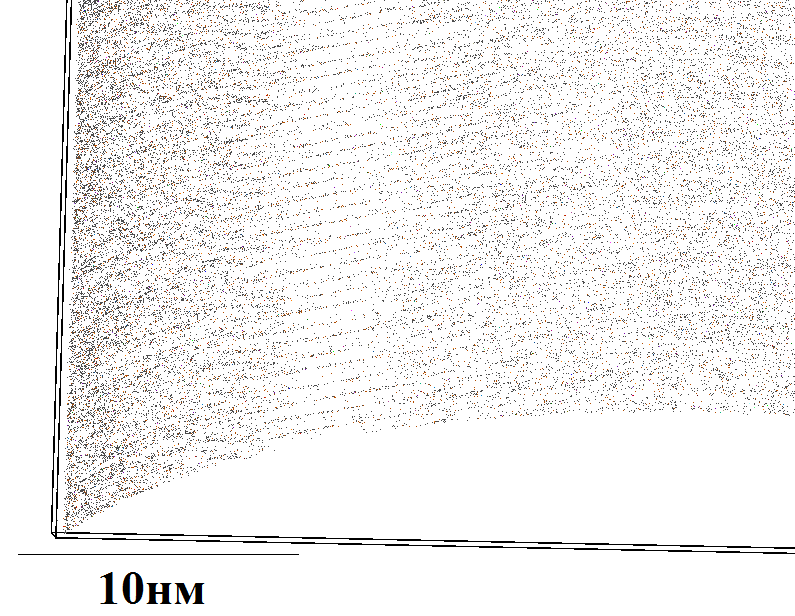
\includegraphics[width=.6\textwidth]{Oleg_3D}
	}
	\caption{Пример атомной карты, на которой видны атомные плоскости в стали Fe-13.5Cr-0.3Ti}
	\label{fig:Oleg_3D}
\end{figure}

Таким образом, показано, что с помощью перебора диапазона мощностей лазера можно получить лучшее качество АЗТ данных. При этом признаками выхода из оптимального диапазона мощности можно считать появление много-зярядных ионов, зярядностей ионов с большим полем испарения и увеличением амплитуды <<тепловых хвостов>>.

После того, как была предварительно оценена мощность лазера, необходимо убедиться, что мощность достаточна для осуществления эксперимента и проверить выставлена ли правильная поляризация. Как было отмечено в литературном обзоре, требуемая поляризация – вдоль оси образца. Для проверки этого факта были произведены эксперименты с изначальной конфигурацией системы, где после сепаратора гармоник был установлен поляризатор, меняющий вертикальную поляризацию на горизонтальную, и без поляризатора, вследствие чего поляризация менялась на противоположную. Полученные масс-спектры в двух режимах приведены на Рисунках \cref{fig:Oleg_polarize_ini} и \cref{fig:Oleg_polarize_final}. Используемый материал - ДУО сталь Fe-13.5Cr-0.3Ti. Мощность лазера – 10 мВт, температура образца – 50 К, нижняя граница потока событий – 200 ат/сек.

\begin{figure}[htb]
	\centerfloat{
		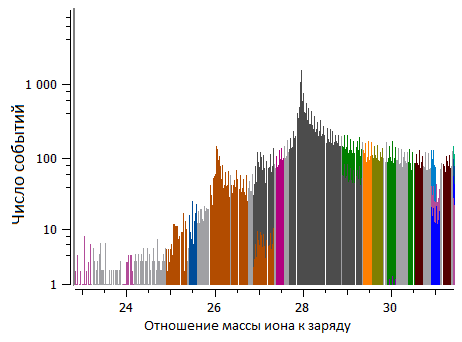
\includegraphics[width=.6\textwidth]{Oleg_polarize_ini}
	}
	\caption{Масс-спектр при предустановленной поляризации (300 тыс. событий)}
	\label{fig:Oleg_polarize_ini}
\end{figure}

\begin{figure}[htb]
	\centerfloat{
		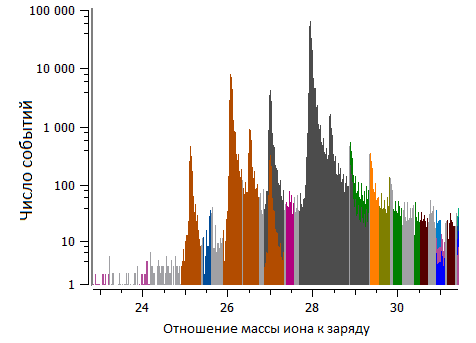
\includegraphics[width=.6\textwidth]{Oleg_polarize_final}
	}
	\caption{Масс-спектр с поляризацией, повернутой на 90 градусов (300 тыс. событий)}
	\label{fig:Oleg_polarize_final}
\end{figure}

Очевидно, что поляризация на Рисунке \cref{fig:Oleg_polarize_ini} не является оптимальной. При смене поляризации разрешение по массе на 10\% высоты выросло с 2 до 237.

\FloatBarrier

\section{Определение оптимальной метрики качества испарения}\label{sec:ch3/sect3}

В ходе сбора данных с одного образца ряд факторов может приводить к изменению условий испарения атомов материала. Например, происходит изменение формы кончика образца (так как он постепенно испаряется), может происходить медленный <<дрейф>>  мощности лазера или фокусировка лазерного излучения может выйти из оптимального положения. Данные изменения приводят к различным отклонениям в испарении, которые будут влиять на результат анализа данных. Следовательно, для проведения количественных исследований необходимо разработать методику поддержания постоянных и воспроизводимых условий испарения в рамках исследования одного образца. В разделе \cref{sec:ch1/sec5} описаны основные используемые метрики для сравнения АЗТ данных. Поскольку ПАЗЛ-3D это новая разработанная установка, то необходимо разработать методику сравнения результатов исследований для обеспечения воспроизводимости получаемых данных.

Для отработки данной методики был выбран сплав Al-3.5Cu-0.2Mn-0.1S~wt\%. Это однородный материал на масштабах нескольких сотен нанометров. Также стоит отметить, что это 4-компонентный сплав, что дает возможность проследить изменения концентраций нескольких элементов друг относительно друга при различных условиях испарения. Исследования проводились при постоянной температуре образца 50 К. Остальные параметры менялись в ходе сбора данных. В начале работы были выбраны несколько различных метрик-кандидатов для оценки пригодности для контроля условий испарения. Ниже приведен список возможных метрик:

\begin{itemize}
	\item Концентрации элементов,
	\item Мощность лазерного излучения,
	\item Доля однократных событий (или общая доля мультисобытий),
	\item Доля мультисобытий одного из элементов,
	\item Соотношение зарядностей основного элемента,
	\item Доля шум до пика основного элемента (10-11 а.е.м.),
	\item Доля шум после пика основного элемента (40-41 а.е.м.).		
\end{itemize}

К метрикам предъявлялось несколько требований. Первое и основное - корректность получаемых концентраций элементов. Второе, не менее важное требование, это возможность вычислять значение выбранной метрики <<in-situ>> в процессе сбора данных. Также требовалась минимальная повторяемость результатов, хотя бы в рамках одного исследования. Для оценки повторяемости значений метрик данные собирались в определенном порядке. Основным варьируемым параметром являлась мощность лазерного излучения. Соответственно, в ходе исследований мощность сначала поэтапно уменьшали, потом увеличивали, затем опять уменьшали. Это позволило оценить возможность воспроизводить условия испарения на протяжении всего сбора данных. В таблицах Приложения \cref{app:B} приведены все параметры проведения исследований и результаты расчета значений выбранных метрик. Далее в работе показаны основные зависимости, которые были обнаружены или наличие которых было подтверждено (ранее они описывались для других атомно-зондовых томографов).

Наиболее очевидной и ожидаемой являлась зависимость детектируемой концентрации от мощности лазерного излучения. Точки зависимости приведены на Рисунках  \cref{fig:params_Conc_Power}, где точки соединены в порядке сбора данных.  Зависимость концентрации элемента практически прямо пропорциональна мощности лазерного излучения. Но в случае другой фокусировки лазера, а следовательно и другой мощности излучения лазера, уже наблюдается нелинейная зависимость (рисунок \cref{fig:params_Conc_Power} б)). Скорее всего есть область оптимума точности сбора данных между слишком малой и слишком большой мощностями лазерного излучения. Данное предположение коррелирует с наблюдаемыми зависимостями качества данных в работе \cite{scbibOptParamsYAFI} (подробно описывалось в разделе \cref{sec:ch1/sec5}).

\begin{figure}[htb]
	\begin{minipage}[b]{0.49\textwidth}\centering
		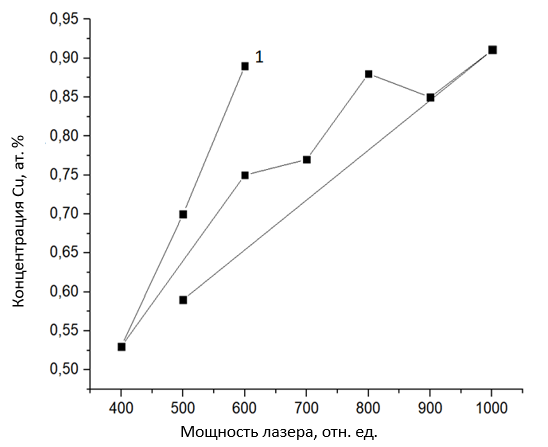
\includegraphics[width=\textwidth]{params_Conc_Power} \\ а)
	\end{minipage}
	\begin{minipage}[b]{0.49\textwidth}\centering
		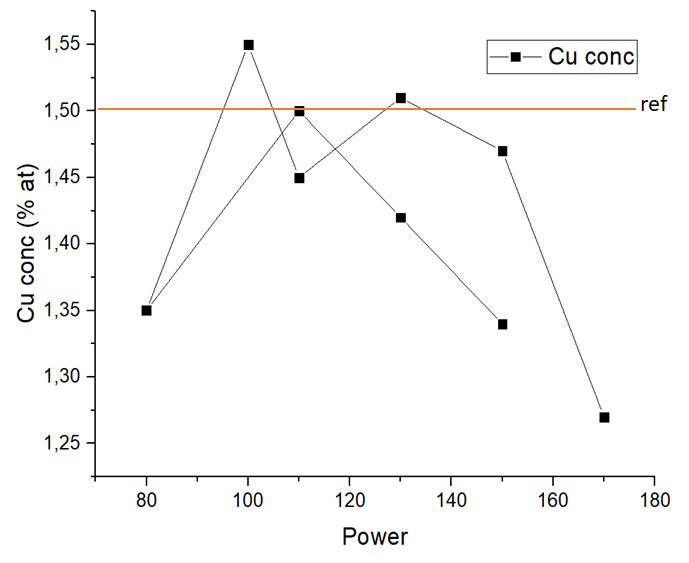
\includegraphics[width=\textwidth]{params_Conc_Power_2} \\ б)
	\end{minipage}
	\caption{Значения концентрации Cu при различной мощности лазерного излучения для двух наборов исследований. Точки соединены в порядке сбора данных. Оранжевой горизонтальной линией на отмечено табличное значение концентрации меди для исследуемого материала}
	\label{fig:params_Conc_Power}
\end{figure}

\FloatBarrier

Важно отметить, что данные для Рисунка \cref{fig:params_Conc_Power} были обработаны уже после проведения исследований. Как выше было неоднократно отмечено, что напрямую концентрации в процессе сбора данных затруднительно вычислять точно, с учетом шума/коррекций/оптимизаций.

Далее изучим другую, более перспективную метрику, основанную на соотношении зарядностей. Поскольку основным элементом в данном материале является алюминий, то была оценена зависимость концентрации меди от отношения $Al^{+}/Al^{++}$ (Рисунок \cref{fig:params_Conc_CSR}).

\begin{figure}[htb]
	\begin{minipage}[b]{0.49\textwidth}\centering
		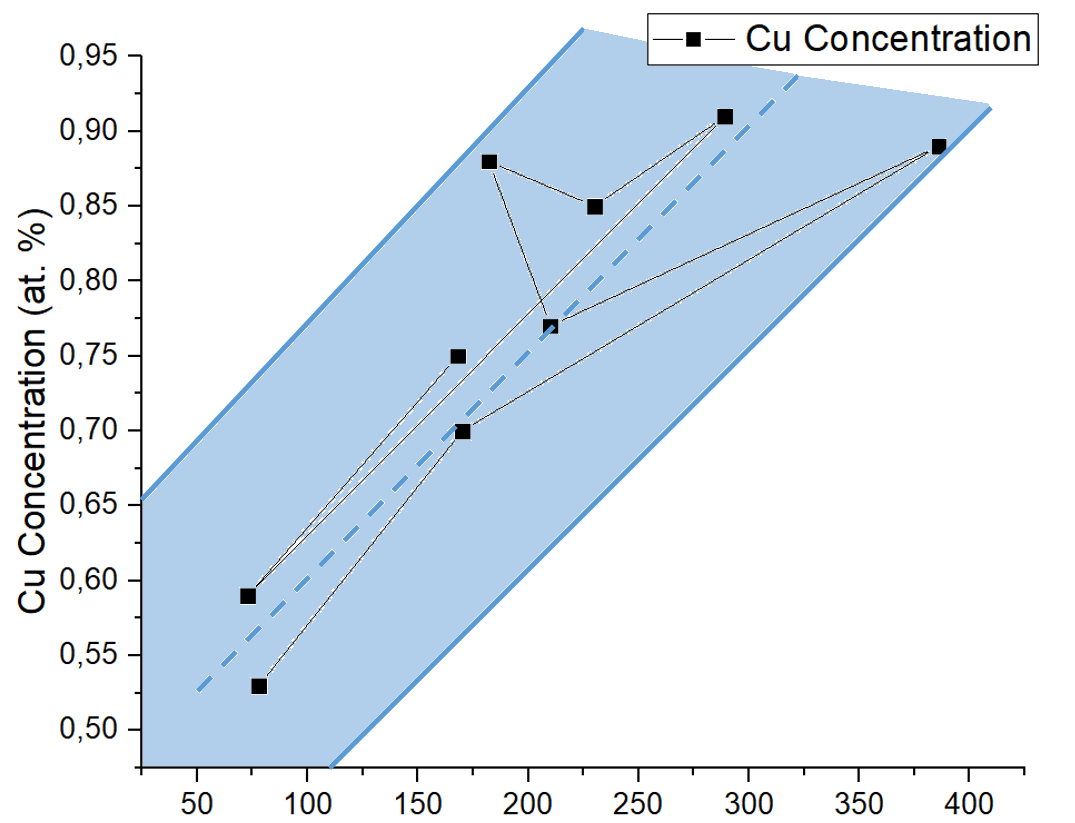
\includegraphics[width=\textwidth]{CSR_1} \\ а)
	\end{minipage}
	\begin{minipage}[b]{0.49\textwidth}\centering
		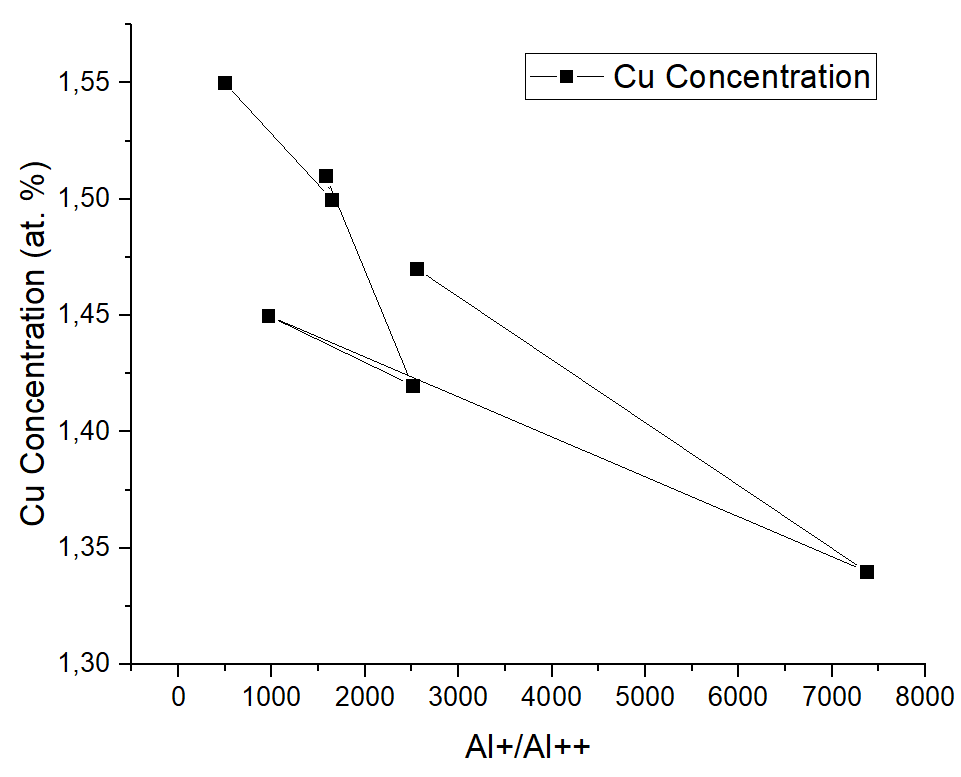
\includegraphics[width=\textwidth]{CSR_2} \\ б)
	\end{minipage}
	\caption{Значения концентрации Cu при различном соотношении зарядностей алюминия для двух наборов исследований. Точки соединены в порядке сбора данных. Пунктирная синяя линия - аппроксимирующая зависимость.}
	\label{fig:params_Conc_CSR}
\end{figure}

На Рисунке \cref{fig:params_Conc_CSR} наглядно видно, что для первого набора данных в области значений $Al^{+}/Al^{++}$ от 75 до 400 концентрация меди не достигает требуемого значения в 1.52 ат. \%, но при этом явно наблюдается воспроизводимость значения концентрации при похожих значениях соотношения зарядностей. Наблюдаемую зависимость можно аппроксимировать линейной функцией ($y = ax + b$) с параметрами a = (11.7 $\pm$ 0.3) * $10^{-4}$, b = 0.53 $\pm$ 0.06 ($R^{2} = 0.67$). При этом для второго набора данных наблюдается противоположный характер зависимости. В этом случае можно также провести аппроксимацию линейной зависимостью с параметрами a = (-2.6 $\pm$ 0.6) * $10^{-5}$, b = 1.53 $\pm$ 0.02 ($R^{2} = 0.72$). Стоит отметить, что во втором наборе данных 2 промежуточные точки практически с идеальной точностью соответствуют табличному значению концентрации меди в данном материале. Аналогичный характер зависимостей наблюдался в работе \cite{Mancini14}, что подтверждает корректность предложенной методики. Для второго набора данных также построены значения концентраций других элементов  в зависимости от соотношения зарядностей алюминия (Рисунок \cref{fig:params_Sn_Mn_O}).

\begin{figure*}
	\centering
	\begin{subfigure}[b]{0.475\textwidth}
		\centering
		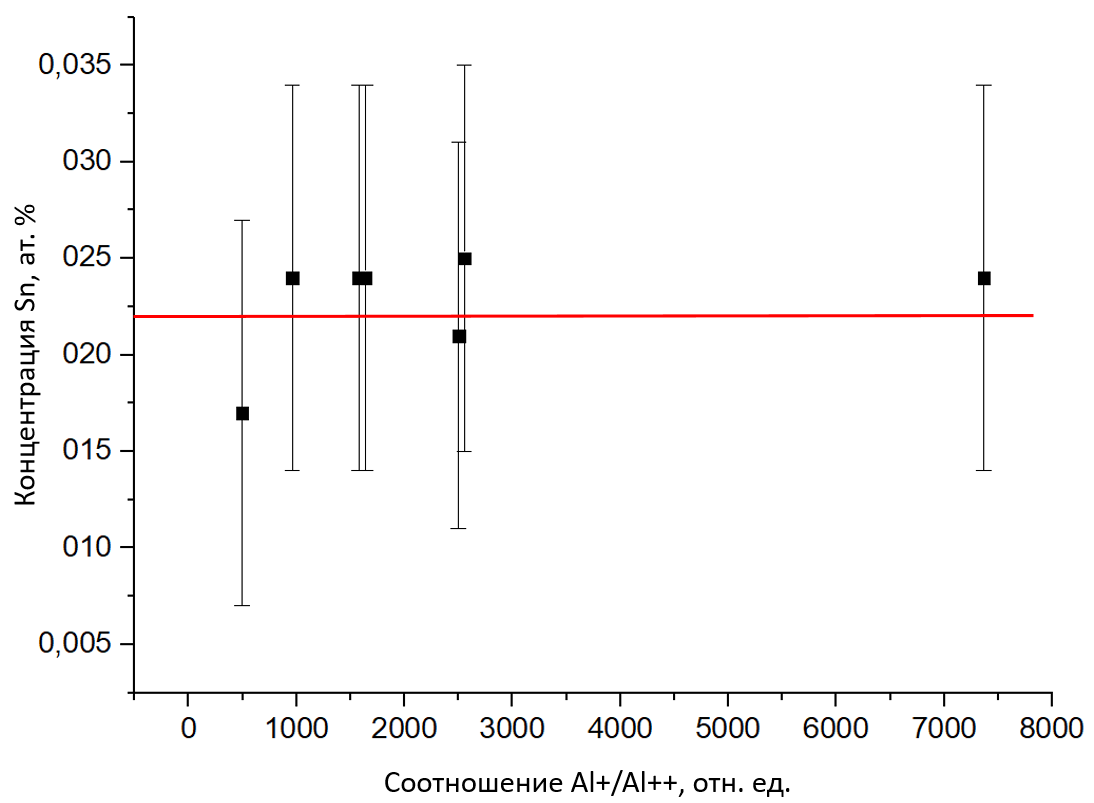
\includegraphics[width=\textwidth]{params_sn_conc}
		\caption{}    
	\end{subfigure}
	\hfill
	\begin{subfigure}[b]{0.475\textwidth}  
		\centering 
		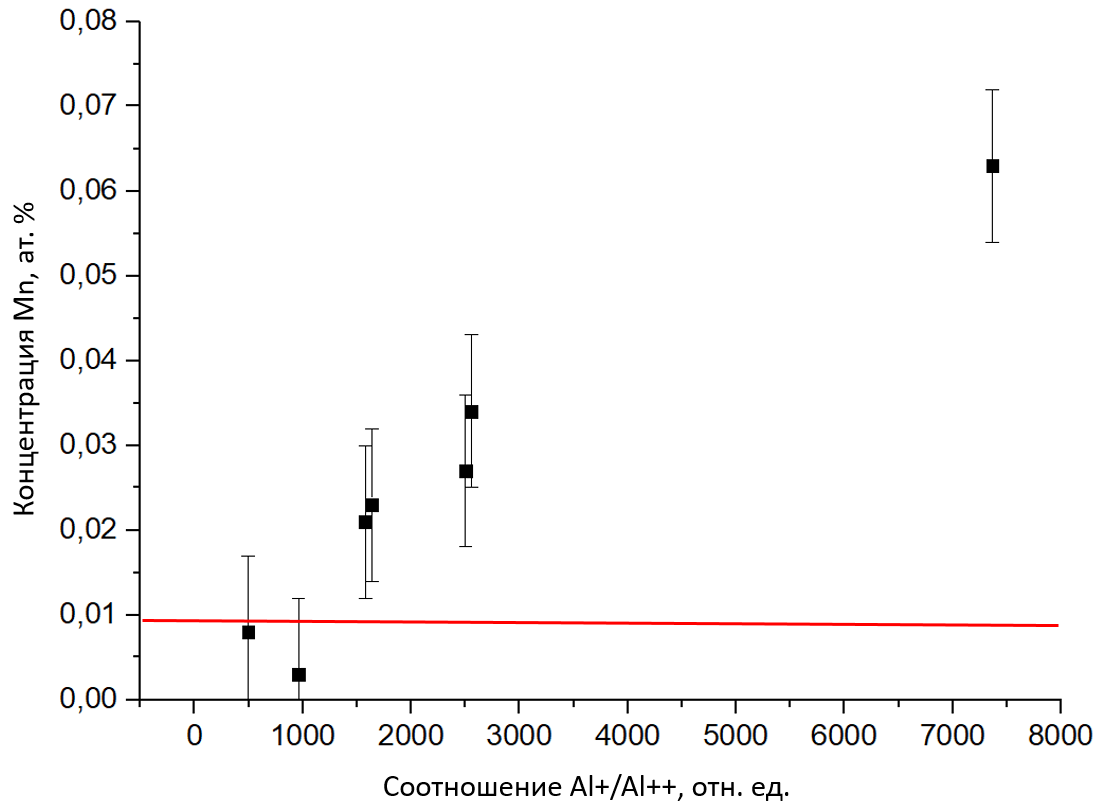
\includegraphics[width=\textwidth]{params_mn_conc}
		\caption{}    
	\end{subfigure}
	\vskip\baselineskip
	\begin{subfigure}[b]{0.475\textwidth}   
		\centering 
		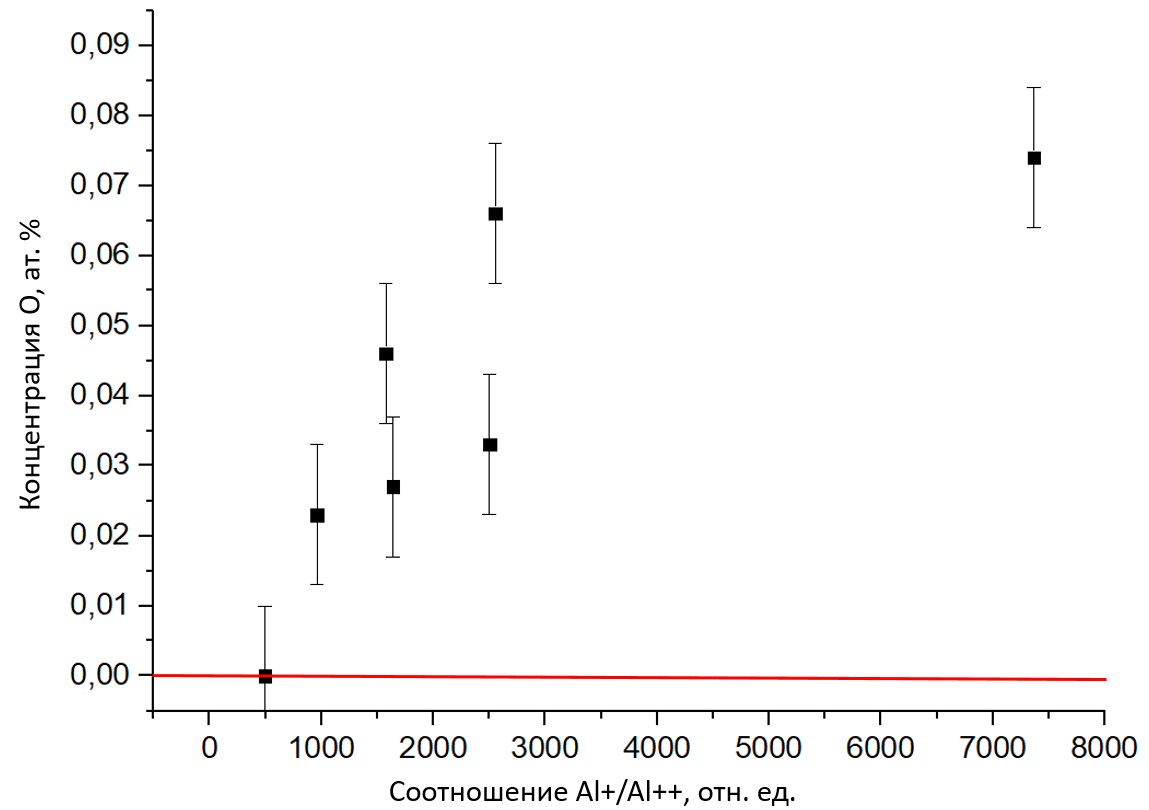
\includegraphics[width=\textwidth]{params_o_conc}
		\caption{}    
	\end{subfigure}
	\hfill
	\caption
	{Значения концентраций Sn (а), Mn (б), O (в) в зависимости от соотношения зарядностей алюминия. Красной линией указаны ожидаемые значения концентрации для исследуемого материала   } 
	\label{fig:params_Sn_Mn_O}
\end{figure*}

Анализируя результаты, показанные на Рисунках \cref{fig:params_Conc_CSR,fig:params_Sn_Mn_O} можно заключить, что для установки ПАЗЛ-3D для алюминиевого сплава Al-3.5Cu-0.2Mn-0.1S~wt\% оптимальным диапазоном значений соотношения зарядностей является промежуток от 300 до 2000 отн. еди. В данном промежутке концентрации меди и олова наиболее близки к табличным значениям. При этом наблюдается малое количество кислорода, наличие которого является артефактом лазерного испарения. Таким образом показано, что соотношение зарядностей основного элемента может служить метрикой качества данных. Показана воспроизводимость результатов исследований с использованием контроля условий испарения по соотношению зарядностей основного элемента.

При оценке зависимости качества АЗТ данных от других метрик было продемонстрировано несколько второстепенных зависимостей (или показано их отсутствие) для сплава Al-3.5Cu-0.2Mn-0.1S~wt\%:

\begin{itemize}
	\item Доля мультисобытий не является воспроизводимой метрикой для АЗТ данных,
	\item Мощность лазерного излучения пропорциональная соотношению зарядностей, но имеет плохую воспроизводимость на разных наборах данных, а следовательно точно не подходит для разных установок (Рисунок \cref{fig:params_Noise_Multi} в)),	
	\item Доля мультисобытий меди имеет тенденцию к снижению с ростом напряжения на образце,
	\item Доля шум до пика основного элемента (10-11 а.е.м.) и доля шум после пика основного элемента (40-41 а.е.м.)	падают с увеличением мощности лазерного излучения и увеличиваются с ростом напряжения на образце (Рисунок \cref{fig:params_Noise_Multi} а) и б)),
	\item Доля мультисобытий меди не является воспроизводимой метрикой для АЗТ данных.	
\end{itemize}

Полученные второстепенные зависимости могут быть важны для более оптимального выбора условий испарения в дальнейших работах по развитию методик исследования алюминиевых сплавов. Также полученные корреляции могут использоваться для лучшей интерпретации данных. Все указанные метрики собраны в Таблице \cref{tab:params_expl}, в которой также приведены основные их особенности как кандидатов для основной метрики качества и воспроизводимости данных.

\begin{figure*}
	\centering
	\begin{subfigure}[b]{0.475\textwidth}
		\centering
		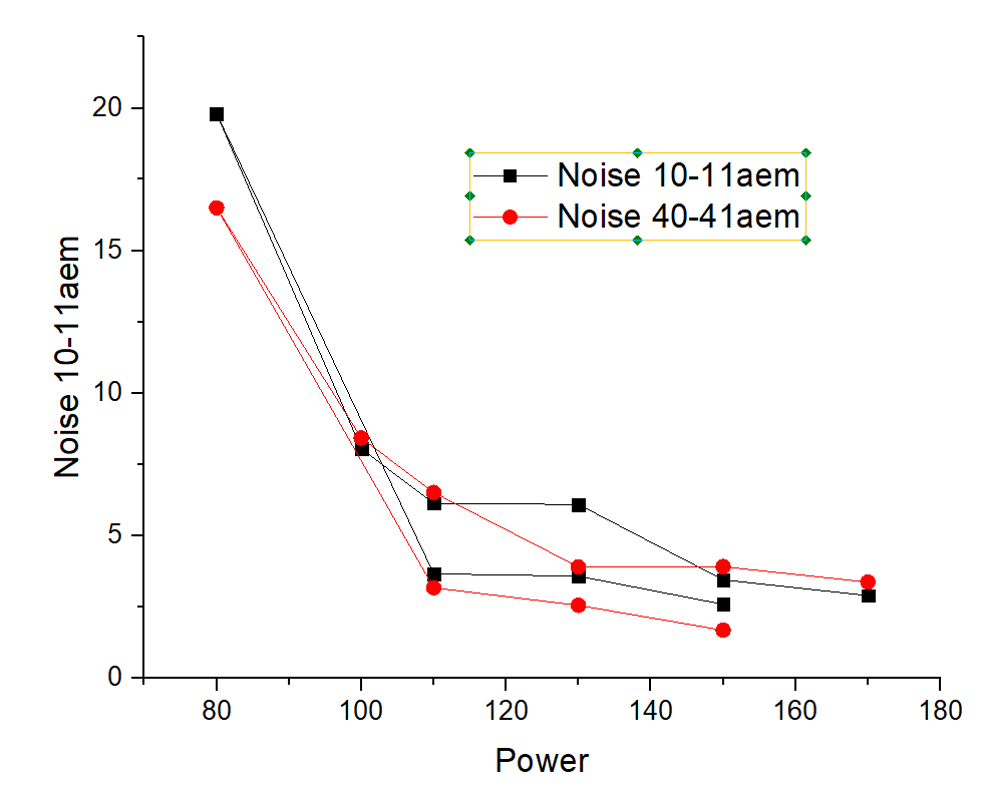
\includegraphics[width=\textwidth]{params_Noise_Power}
		\caption{}    
	\end{subfigure}
	\hfill
	\begin{subfigure}[b]{0.475\textwidth}  
		\centering 
		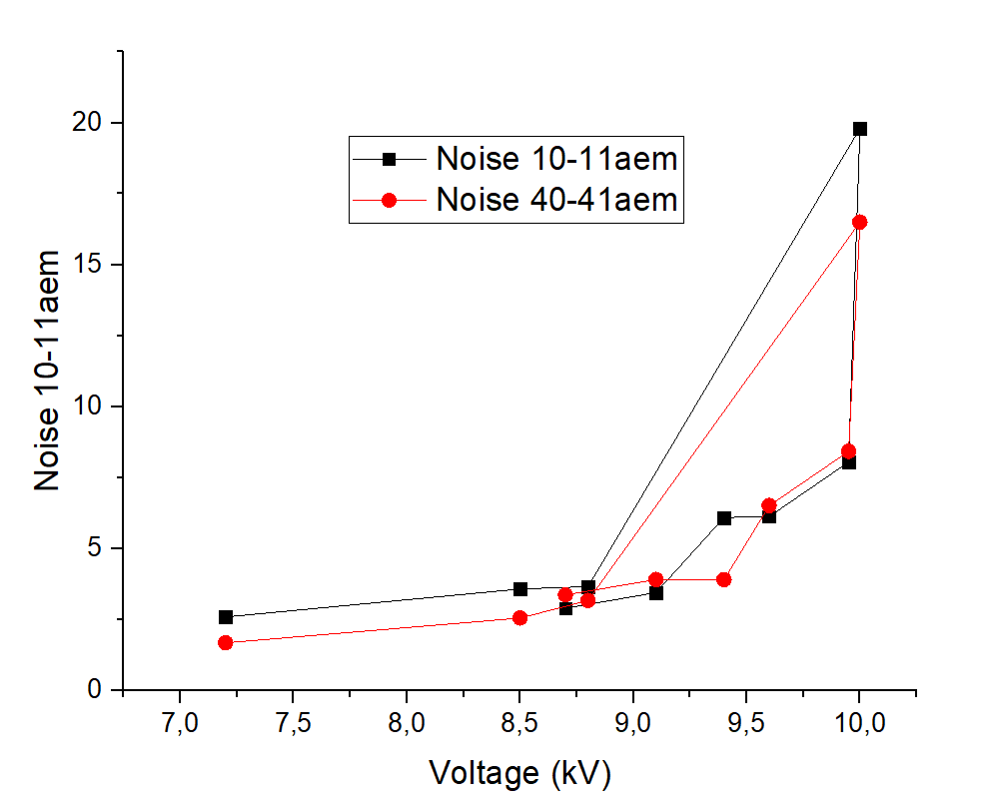
\includegraphics[width=\textwidth]{params_Noise_Voltage}
		\caption{}    
	\end{subfigure}
	\vskip\baselineskip
	\begin{subfigure}[b]{0.475\textwidth}   
		\centering 
		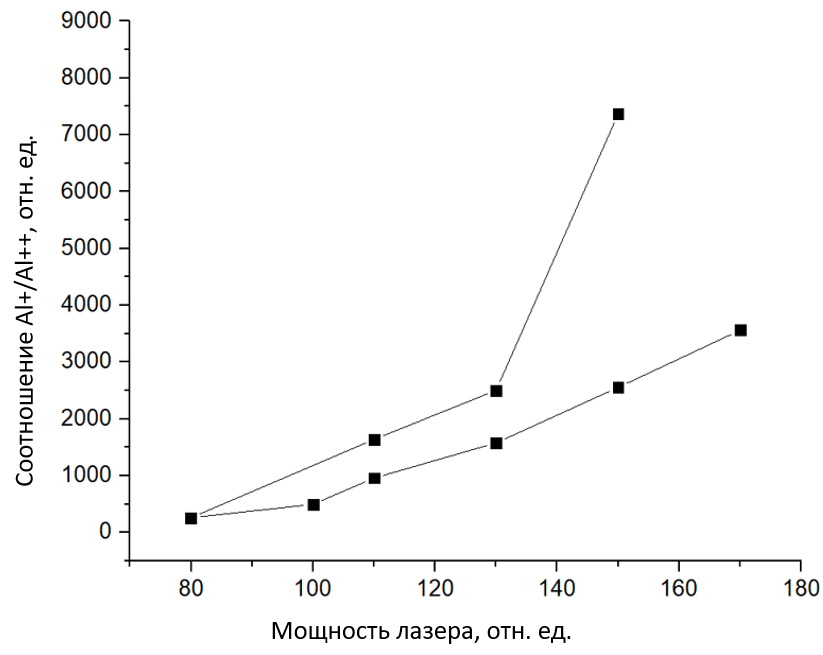
\includegraphics[width=\textwidth]{params_CSR_Power}
		\caption{}    
	\end{subfigure}
	\hfill
	\caption
	{а) - Значения шума до и после пика основного элемента от мощности лазерного излучения. б) - Значения шума до и после пика основного элемента от напряжения на образце. в) Значения соотношения зарядностей в зависимости от мощности лазерного излучения. На всех рисунках точки соединены в порядке сбора данных} 
	\label{fig:params_Noise_Multi}
\end{figure*}

\begin{table} [htb]
	\centering
	\caption{Метрики качества атомно-зондовых данных}
	\label{tab:params_expl}
	\begin{SingleSpace}
		\begin{tabularx}{\textwidth} {| X | X | X | X |}
			\hline
			Наименование & Описание/ комментарии & Возможная интерпретация & Минусы  \\ \hline
			Однократные события & {Доля однократных событий ко всем событиям}  & {Чем больше - тем проще расшифровывать данные}  & {Нет прямой корреляции с концентрациями}              \\ \hline
			Мощность лазера & {Легко измеряется/ меняется в процессе исследования}  & {-}  & {нет повторяемости от образца к образцу}              \\ \hline
			Доля мультисобытий Cu & Возможная метрика сложности точности определения концентрации & Чем меньше - тем лучше & Нет прямой корреляции с концентрациями          \\ \hline		
			Шум до пиков основного элемента сплава      & Доля атомов с массами от 10 до 11 а.е.м. & Чем больше мощность лазера, тем меньше шума, чем выше напряжение, тем больше шума  & Нет прямой корреляции с концентрациями               \\ \hline
			Шум после пиков основного элемента сплава     & Доля атомов с массами от 40 до 41 а.е.м. & Чем больше мощность лазера, тем меньше шума, чем выше напряжение, тем больше шума  & Нет прямой корреляции с концентрациями             \\ \hline
			Концентрации  & -   &  -   & Расчет невозможен в реальном времени  \\ \hline			
			Соотношение зарядностей основного элемента Al$^+$/Al$^{++}$, отн. ед.    & Возможна оценка по предварительному масс-спектру, без оптимизации   & Есть значимая зависимость и повторяемость концентраций от соотношения зарядностей  & Может отличаться для разных материалов   \\ \hline
		\end{tabularx}
	\end{SingleSpace}
\end{table}

\FloatBarrier
Таким образом, в данном разделе продемонстрирована методика выбора метрики качества и воспроизводимости АЗТ данных для алюминиевых сплавов. Показано, что предпочтительная метрика, основанная на соотношение зарядностей для основного химического элемента материала. Основываясь на том, что сохранение соотношения зарядностей основного химического элемента обеспечивают воспроизводимость результатов АЗТ исследований (концентрации близки к ожидаемым), можно заключить, что методика поиска оптимальных параметров испарения включает следующее:

\begin{itemize}
	\item сбор набора АЗТ данных при различных соотношения зарядностей основного химического элемента,
	\item расчет концентрации всех элементов,	
	\item (дополнительно) проверка данных на отсутствие артефактов испарения (например, наличия кислорода, не входящего в состав материала),
	\item в случае неполучения целевых значений концентраций или наличия большого числа артефактов проверка более широкого диапазона значений соотношений зарядностей,
	\item выбор диапазона значений соотношений зарадностей, при котором концентрации наиболее близки к целевым значениям и при этом наблюдается минимальное количество артефактов испарения.	
\end{itemize}

В дальнейших исследованиях сплавов данного типа можно придерживаться выбранного диапазона значений соотношений зарядностей.

\FloatBarrier



\section{Методика коррекции восстановления атомно-зондовых данных с учетом атомной плотности}\label{sec:ch3/sect5}

В атомно-зондовой томографии на качество данных влияет множество факторов на каждом из этапов работы с данными. В ходе сбора данных на установке необходимо следовать определенным методикам сбора данных (например, см. Раздел \cref{sec:ch3/sect4}). Восстановление АЗТ данных также является сложной процедурой, которая может существенно повлиять на количественные характеристики результатов исследования. На точность восстановления 3D координат атомов в АЗТ данных зависит от параметров и конфигурации АЗТ установки и от алгоритма восстановления координат. Для реконструкции 3D координат можно использовать несколько алгоритмов. Наиболее значимым различием между ними является выбор способа учета изменения радиуса кончика образца. В ПО <<КВАНТМ-3D>> используется алгоритм восстановления 3D данных, предложенный Bas. Как было указано в Разделе \cref{sec:ch1/sec3}, одной из его отличительной особенностью является то, что радиус кончика образца пропорционален напряжению на образце. Исходя из формул \cref{eq:equation11,eq:equation12} можно выделить следующие параметры, зависящие от материала, формы образца или установки АЗТ, которые будут влиять на 3D восстановление:

\begin{itemize}[beginpenalty=10000] % https://tex.stackexchange.com/a/476052/104425
	\item фактор сжатия изображения (далее ICF или $\xi$);
	\item длина пролета иона;
	\item полевой фактор (далее $k_f$);
	\item атомный объем ($\Omega$);
	\item эффективность детектирования.
\end{itemize}

Длина пролета учитывается в оптимизационных алгоритмах <<КВАНТМ-3D>> \cite{Shutov18,Shutov19}. Атомный объем указывается индивидуально для каждого сорта атомов. Два эти параметра практически в автоматическом режиме учитываются при восстановлении 3D координат. Эффективность детектирования принимается постоянной в рамках исследований на одной и той же установке. Оставшиеся параметры ICF и $k_f$ могут изменяться в ходе сбора данных. Например, в работах \cite{Geiser09,Gipson08} изучается зависимость ICF от формы образца или электростатической системы установки. При этом проводились калибровочные исследования для измерения зависимостей ICF и $k_f$ для разных типов установок: ECOTAP \cite{Geiser09}, LAWATAP \cite{Renaud03}, LEAP 3000 \cite{Renaud06}. Естественно, в дополнение в экспериментальным данным проводились исследования по моделированию зависимостей параметров восстановления данных от условий испарения \cite{Vurpillot11,Miller14,Hatzoglou19}. Данный факт показывает необходимость вы определении указанных зависимостей для ПАЗЛ-3D.


Для определения зависимостей полевого фактора и фактора сжатия изображения на первом этапе рассмотрим возможное влияние параметров ICF и $k_f$ на  характер восстановления 3D координат. В рамках методики реконструкции координат атомов, предложенной в работе Bas \cite{Bas95}, можно дополнительно использовать стереографическую проекцию координат атомов на поверхность образца. Тогда латеральные координаты X и Y будут определяться по следующим выражениям:

\begin{equation}
	\label{eq:equation3_1}
	X = R \sin{\phi}\sin{\theta},	
\end{equation}

\begin{equation}
	\label{eq:equation3_2}
	Y = R \cos{\phi}\sin{\theta},	
\end{equation}

где $\theta$ - полярный угол, $\phi$ - азимутальный угол, R - радиус кончика образца. Радиус вершины образца определяется по выражению \cref{eq:equation11}.  Определение угла $\theta$ показано на Рисунке \cref{fig:p3_projection}.

\begin{figure}[htb]
	\centerfloat{
		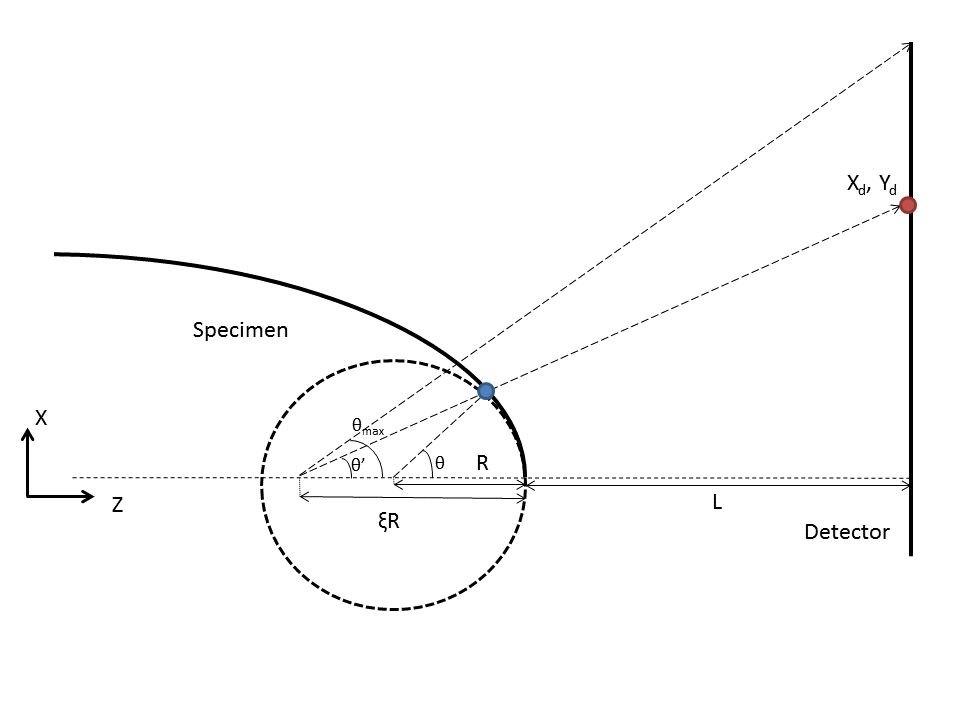
\includegraphics[width=\textwidth]{p3_projection}
	}
	\caption{Схема стереографической проекции координат атома на вершину образца \cite{scbibDensity}. Показано определение реального угла испарения иона $\theta$ и наблюдаемого угла испарения иона $\theta$'.}
	\label{fig:p3_projection}
\end{figure} 

Угол $\theta$' рассчитывается по известным значениям расстояния между образцом и детектором и значениями координат иона на детекторе $X_p, Y_p$. Прямая связь между двумя углами $\theta$ и $\theta$' и координатой Z может быть получена как:

\begin{equation}
	\label{eq:equation3_4}
	\theta = \theta' + \arcsin(\xi - 1)\sin{\theta'},
\end{equation}

\begin{equation}
	\label{eq:equation3_5}
	z_i = \frac{\Omega N_i}{Q R^2 \pi 2 {\sin^2(\theta_{max})}} + R (1- \cos{\theta}),
\end{equation}

где $\theta$ - исходный угол вылета иона, который представляет собой реальный угол проекции, $\theta$' - угол, наблюдаемый после сжатия траекторий иона, $\xi$ - фактор сжатия изображения ICF, Q - эффективность обнаружения, $N_i$ - номер обнаруженного атома. Угол $\theta_{max}$ - это максимальный угол обнаружения атомов. Важно отметить, что углы $\theta$ и $\theta$' могут изменяться в пределах от 0 до $\pi/2$.

Далее рассмотрим влияние $k_f$ и ICF на характер изменения координат X, Y и Z более детально. Из выражений \cref{eq:equation3_1,eq:equation3_2,eq:equation3_4} видно, что координаты X и Y  пропорциональны величине ICF в пределах допустимых значений угла $\theta$ от 0 до $\pi/2$. В выражении \cref{eq:equation3_5} Z координата равна сумме двух слагаемых. Первое отвечает за смещение по оси Z вдоль всего образца в зависимости от номера испаренного атома. Второе слагаемое определяется степенью кривизны поверхности, с которой был испарен атом. Фактор сжатия изображения фигурирует только в части определения кривизны поверхности образца. Соответственно, смещение атома по координате Z практически не зависит от ICF. Полевой фактор, в свою очередь, влияет и на координаты X, Y, и на координату Z, поскольку $k_f$ присутствует в формуле определения радиуса~\cref{eq:equation11}.

Для наглядной демонстрации характера зависимостей координат атомов от $k_f$ и ICF был восстановлен один и тот же объем атомов при различных значениях $k_f$ и ICF. На Рисунке \cref{fig:p3_3Dparts} показаны атомные карты образца, восстановленные при разных параметрах восстановления.

\begin{figure}[htb]
	\centerfloat{
		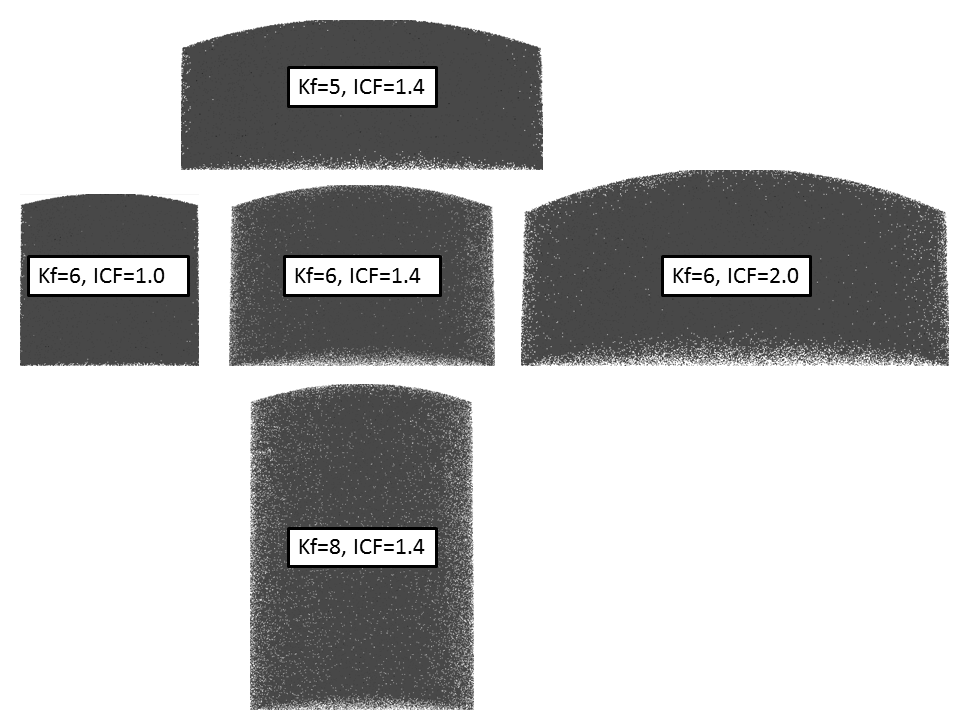
\includegraphics[width=\textwidth]{p3_3Dparts}
	}
	\caption{Атомные карты реконструируемого образца с различными значениях полевого фактора ($k_f$) и фактора сжатия изображения (ICF) \cite{scbibDensity}}
	\label{fig:p3_3Dparts}
\end{figure}

На Рисунке \cref{fig:p3_3Dparts} видно, что при неизменном $k_f$, ICF  влияет только на X, Y координаты и на кривизну поверхности образца. Общая высота образца остается практически низменной. В свою очередь, при постоянном ICF, полевой фактор значительно изменяет все линейные размеры реконструируемого объема. В работе \cite{scbibDensity} было высказано предположение, что изменение полевого фактора не меняет плотность атомов при восстановлении данных. Для проверки данного предположения можно рассчитать значения плотности атомов при различных значения полевого фактора и фактора сжатия изображения (см.~Рисунок~\cref{fig:p3_ICF}).

\begin{figure}[htb]
	\begin{minipage}[b][][b]{0.49\textwidth}\centering
		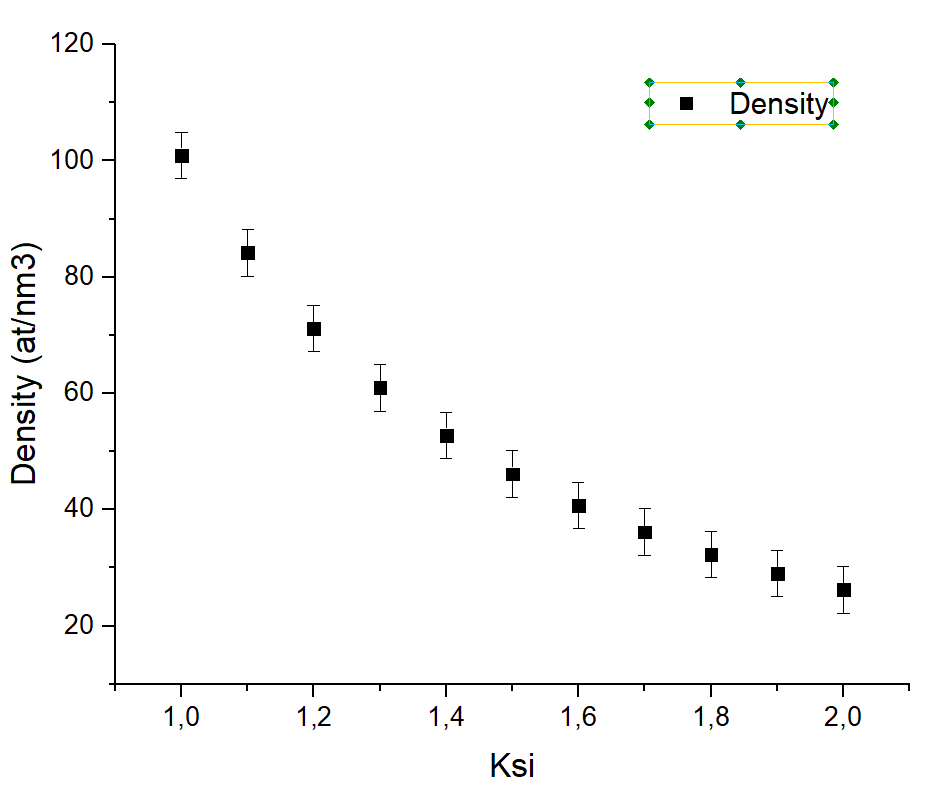
\includegraphics[width=\textwidth]{p3_ICFvsKsi} \\ а)
	\end{minipage}
	%\hfill
	\begin{minipage}[b][][b]{0.49\textwidth}\centering
		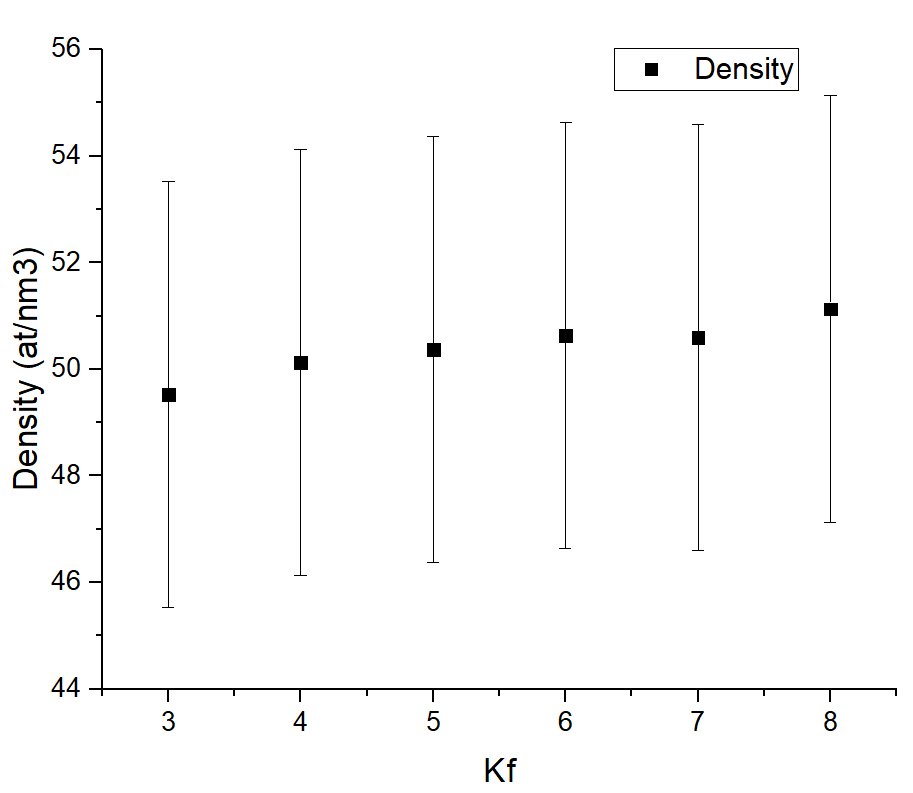
\includegraphics[width=\textwidth]{p3_ICFvskf} \\ б)
	\end{minipage}
	\caption{Значения плотности при различных значениях ICF (а). Значения плотности атомов при различных значениях $k_f$ (б) \cite{scbibDensity}}
	\label{fig:p3_ICF}
\end{figure}

Исходя из допущения, что исследуемый материал имеет постоянную плотность вещества, то есть не имеет включений или объемная доля включений невелика, то плотность атомов можно принять как постоянную величину для всего исследуемого объема. Далее, опираясь на методику определения точности восстановления координат из Раздела \cref{sec:ch3/sect1}, можно рассмотреть следующую методику поиска зависимостей ICF и $k_f$:

\begin{enumerate}[beginpenalty=10000] % https://tex.stackexchange.com/a/476052/104425
	\item Допустим, что плотность атомов постоянна и известна заранее для исследуемого материала, также считаем, что расстояния между атомными плоскостями, соответствующие одному кристаллографическому выходу, постоянны и известны;
	\item Зная плотность атомов подбираем такое значение ICF, чтобы плотность реконструируемого объема совпадала с известной плотностью;
	\item Полевой фактор определяем исходя из трех возможных вариантов:
	\begin{itemize} [beginpenalty=10000]
		\item Если в исследуемом объеме присутствуют включения, и форма этих включений известна (например, зоны Гинье-Престона), то $k_f$ выбирается, так, чтобы форма включений соответствовала ожидаемой;
		\item Если в исследуемом объеме нет включений, то $k_f$ выбирается близким к значениям полевого фактора, выбранных в аналогичных исследованиях;
		\item Если в исследуемом объеме можно различить атомные плоскости, то $k_f$ выбирается таким, чтобы расстояния между атомными плоскостями были одинаковыми во всем объеме данных и наиболее близки к табличному значению.
	\end{itemize}
\end{enumerate}

Стоит отметить, что согласно работам групп Gault \cite{Gault11_Loi}, Loi \cite{Loi13} и Da Costa \cite{Hatzoglou19}, можно предположить, что ICF и $k_f$, найденные для чистых материалов (в которых возможна калибровка по межплоскостным расстояниям), будут одинаковыми для соответствующих сплавов.

Для экспериментального определения значений полевого фактора и фактора сжатия изображений были проведены калибровочные исследования. АЗТ анализ проводился на установке ПАЗЛ-3D. В качестве материалов для исследования выбраны алюминий и вольфрам с объемноцентрированной и гранецентрированной кубической кристаллической структурой соответственно. Исследования проводились при следующих условиях:
\begin{itemize}
	\item температура образца 22 К;
	\item скорость сбора данных от 2 до 6 атомов на 1000 лазерных импульсов;
	\item энергия лазерного импульса от 5 до 10 мВт;
	\item частота лазерных импульсов 25 кГц;
	\item длина волны лазера 515 нм.
\end{itemize} 

Режим испарения поддерживался согласно методике описанной в работе Разницына \cite{scbibOptParamsYAFI}. Реконструкция данных проводилась с помощью программы <<КВАНТМ-3D>> версии 1.5.7. При восстановлении масс-спектра использовалась процедура автоматической калибровки и оптимизации \cite{Shutov19}. Исследования и проверка работоспособности методики проводились на 12 образцах вольфрама и алюминия. Для удобства оценки расстояния между плоскостями атомов был разработан специальный инструмент в программном обеспечении <<KNN-cryst>>. Работа данного инструмента базируется на построении распределения ближайших соседей K порядка \cite{GaultBOOK}, где K принимает значения от 10 до 30 в зависимости от выбора пользователя. <<KNN-cryst>> считает расстояния до ближайших соседей только по Z координате. Ось Z выбрана, поскольку вдоль неё чаще всего наблюдаются атомные плоскости. В случае, если в анализируемом объеме есть атомные плоскости, разработанный инструмент <<увидит>> некоторую периодическую функцию расстояний между ближайшими соседями. Пример показан на Рисунке \cref{fig:p3_atomiccount_distance}. Для визуализации линейной плотности в программе <<КВАНТМ-3D>> модифицирован модуль линейных концентраций. В новой версии возможна визуализация линейной плотности вдоль оси Z, по аналогии с концентрациями, с возможностью выбора шага усреднения и параметров сглаживания.

Для оценки изотропности плотности атомов в объеме рассчитаны значения плотности вдоль оси Z образца алюминия (см. Рисунок \cref{fig:p3_Density_vs_depth}, расчет плотности по стандартному протоколу). 

На Рисунке \cref{fig:p3_Density_vs_depth} видно, что с изменением глубины - меняется значение плотности. Это позволяет предположить, что для корректного восстановления АЗТ данных необходимо внести поправки, связанные с координатой Z, в протокол реконструкции 3D данных. Далее будет описана разработка Протокола динамической реконструкции по плотности материала (ПДРП??). Как выше было сказано, ICF практически не оказывает влияния на Z координату, следовательно, в данном протоколе будет динамически изменяться значение фактора поля.

Исходя из выражений \cref{eq:equation11,eq:equation3_5} и вышеописанных допущений о постоянной плотности, можно заключить, что необходимо найти зависимость полевого фактора от напряжения на образце. Для поиска данной зависимости необходимо разбить объем данных на небольшие части. Для каждой части подобрать такое значение $k_f$, чтобы значение межплоскостных расстояний было наиболее близко к теоретическому. Естественно для калибровки необходимо использовать материал, в котором можно наблюдать атомные плоскости с помощью АЗТ методики. Теоретические значения межплоскостных расстояний можно найти в книге Gault \cite{GaultBOOK}. Из той же книги были использованы карты выходов кристаллографических направлений для определения типа выходов по картам полевого испарения.

\begin{figure}[htb]
	\centerfloat{
		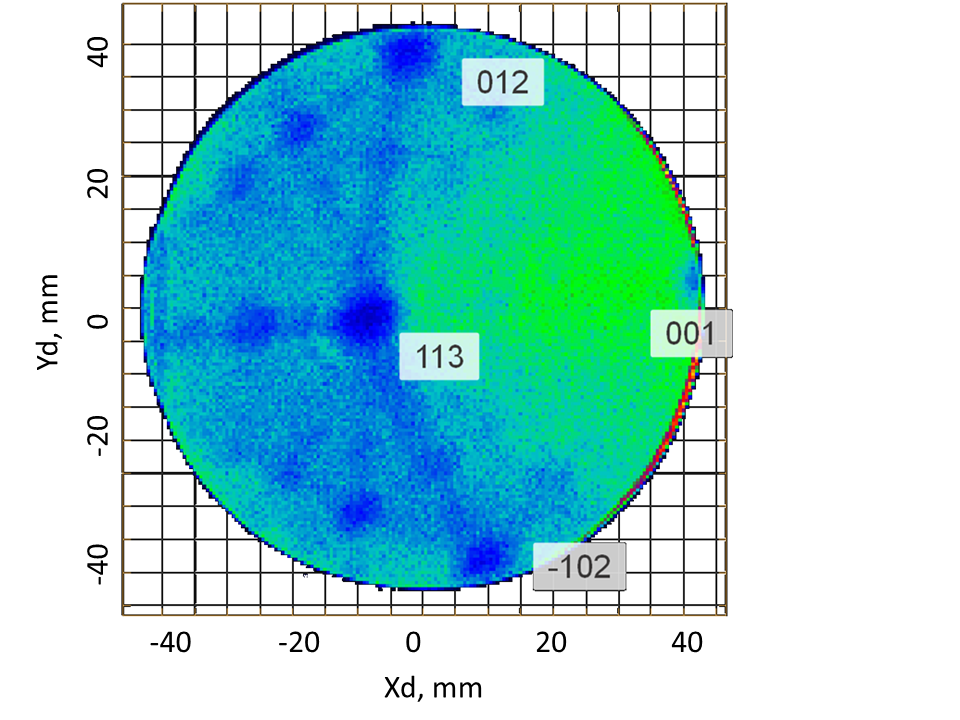
\includegraphics[width=\textwidth]{p3_Alion}
	}
	\caption{Карты полевой десорбции алюминиевого образца. Указаны кристаллографические направления \cite{scbibDensity}}
	\label{fig:p3_Alion}
\end{figure} 

На Рисунке \cref{fig:p3_Alion} показана карта полевого испарения с детектора ПАЗЛ-3D при исследовании алюминиевого образца. Для расчета межплоскостных расстояний был использован выход {113}, поскольку он находится практически в центре детектора, а это значит, что координаты атомов в нем имеют наименьшие искажения. Согласно книге Gault для кристаллографического выхода алюминия {113} расстояние между плоскостями атомов примерно равно 1.2 \r{A}. Выбор разбиения объема на части основывался на требовании получить в каждой части набор из 10-30 плоскостей атомов для более точного определения межплоскостного расстояния. Напряжение для каждой части считалось практически постоянным и равным напряжению в начале сегмента. Полученные значения $k_f$ при различных напряжениях для алюминиевого образца показаны на Рисунке \cref{fig:p3_kf_vs_voltage}. 

\begin{figure}[htb]
	\centerfloat{
		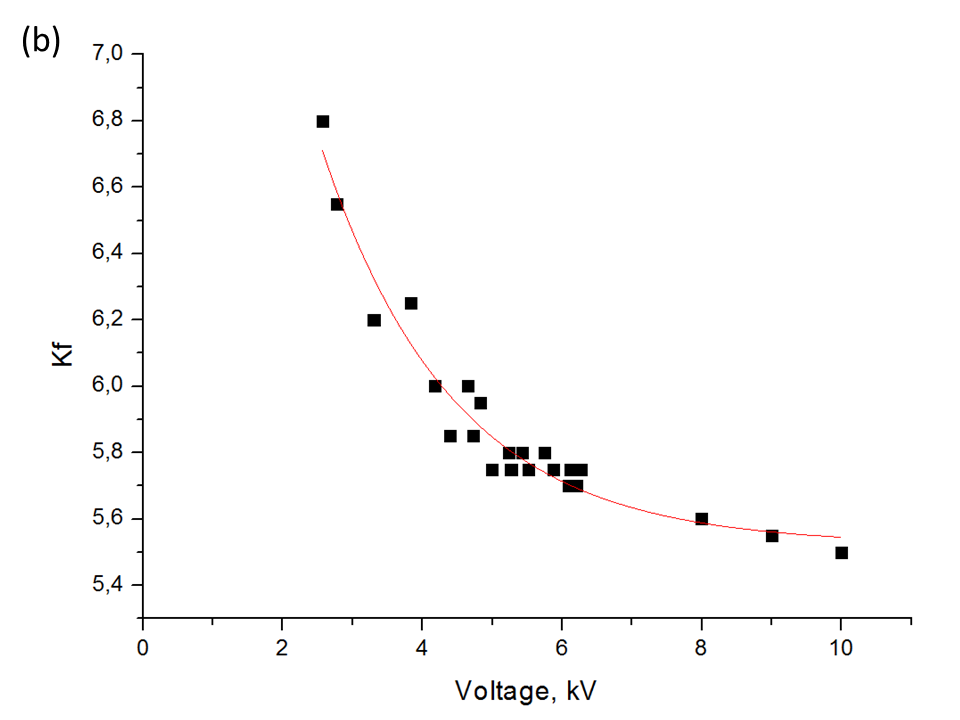
\includegraphics[width=\textwidth]{p3_kf_vs_voltage}
	}
	\caption{Экспериментальные данные $k_f$ \cite{scbibDensity}, полученные для алюминиевого образца (черные точки) и наилучшая аппроксимирующая кривая (красная линия)}
	\label{fig:p3_kf_vs_voltage}
\end{figure} 

Для полученного массива значений $k_f$ и напряжений была проведена аппроксимация экспоненциальной функцией:

\begin{equation}
	\label{eq:equation3_n}
	k_f = (10 - C) + Ce^{-5.3 U 10^{-4}},
\end{equation} 

где C - константа подгонки, U - напряжение на образце. Похожая функция использовалась в работах \cite{Hatzoglou19} и \cite{Loi13}. Различия в зависимостях, возможно, обусловлено различным электростатическим окружением образца в разных установках атомно-зондовой томографии. Значение подгоночной константы для алюминия равно 5.5, а для вольфрама - 4.5. Значимых зависимостей полевого фактора от угла раствора образца или начальным радиусом вершины образца не обнаружено. На Рисунке \cref{fig:p3_PlanesDistance_depth} показаны значения межплоскостных расстояний рассчитанные при использовании разных протоколов реконструкции данных для образца из алюминия. Видно, что  расстояния между плоскостями атомов,  полученные с помощью предлагаемого динамического протокола восстановления, довольно точно совпадают с теоретическим значение.

\begin{figure}[htb]
	\centerfloat{
		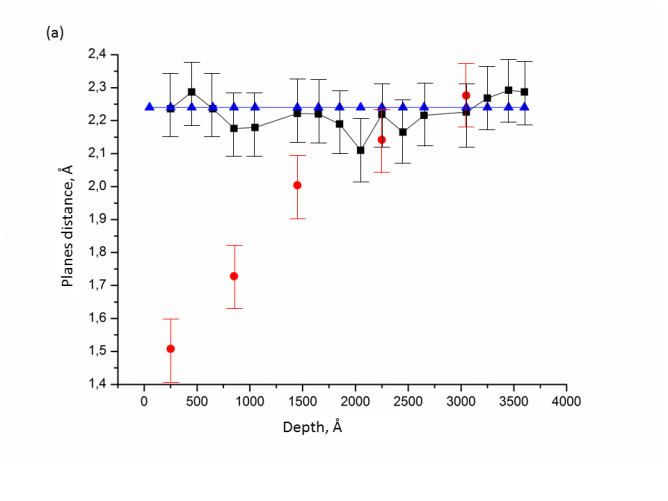
\includegraphics[width=\textwidth]{p3_PlanesDistance_depth}
	}
	\caption{Значения расстояний между атомными плоскостями в зависимости от глубины по оси Z образца из алюминия \cite{scbibDensity}, полученное стандартным протоколом реконструкции (красный), динамическим протоколом $k_f$ (черный). Синим отмечено теоретическое значение межплоскостного расстояния алюминия.}
	\label{fig:p3_PlanesDistance_depth}
\end{figure}

Как выше было указанно, значение ICF влияет на плотность атомов в реконструируемом объеме. Следовательно, определить значение фактора сжатия изображения можно с помощью простого перебора диапазона допустимых значений ICF, с последующим выбором наиболее близкого значения к теоретическому. Допустимые значения ICF находятся в диапазоне от 1 до 2 отн.ед. Для более точного определения значений ICF в зависимости от напряжения на образце необходимо проделать туже процедуру, что и для поиска $k_f$. Объем данных делится по оси Z на небольшие части, для каждой из них методом перебора находится оптимальное значение ICF. В результате был получен набор значений фактора сжатия изображений и напряжений, который аппроксимировался линейной зависимостью. Полученный характер зависимости отличается аналогичных зависимостей, полученных в работах \cite{Hatzoglou19, Gault11_Loi}. Данное отличие связано с использованием разных типов испарения в установках атомно-зондовой томографии. В ПАЗЛ-3D используется лазерное испарение, а в аналогичных работах используются установки с лазерным испарением и/или локальным электродом.

На Рисунке \cref{fig:p3_Density_vs_depth} показаны значения плотности каждой части объема в зависимости от положения по оси Z образца из алюминия. Видно, что с помощью Протокола динамической реконструкции по плотности материала (ПДРП??) удалось нивелировать понизительную тенденцию в реконструкции данных. При это сохраняются отклонения плотности атомов от целевого значения на значимые величины. Предположительно это связано с не идеальной формой кончика образца.

\begin{figure}[htb]
	\centerfloat{
		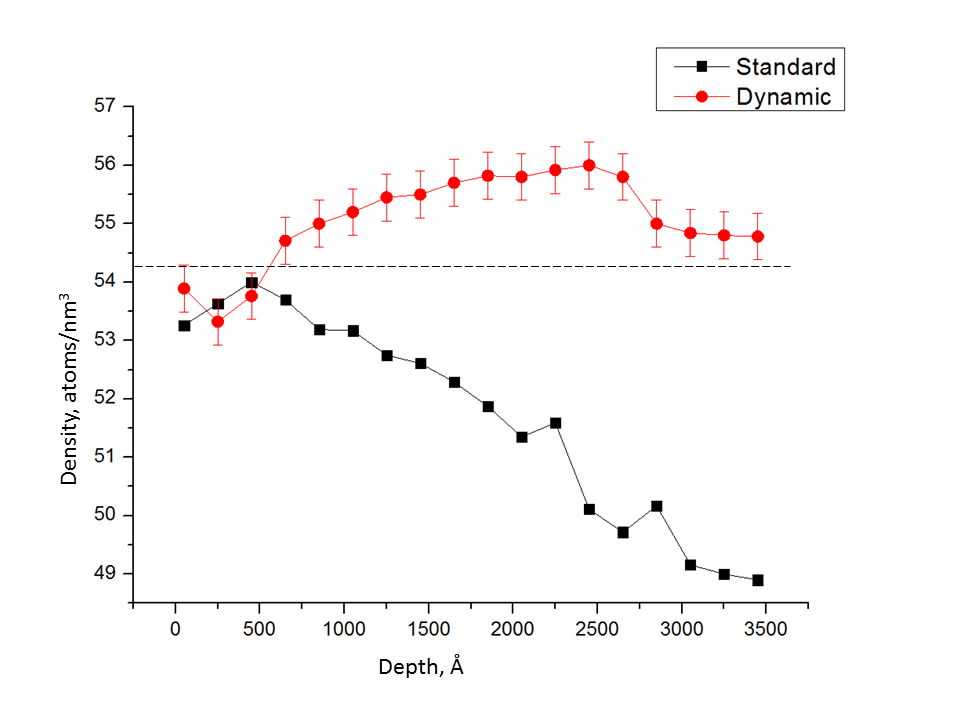
\includegraphics[width=\textwidth]{p3_Density_vs_depth}
	}
	\caption{Значения линейной плотности атомов в образце из алюминия вдоль оси Z образца \cite{scbibDensity}, полученная по стандартному протоколу (черные точки) и по Протоколу динамической реконструкции по плотности материала (ПДРП??) (красные точки). Пунктирная линия показывает ожидаемую плотность алюминия.}
	\label{fig:p3_Density_vs_depth}
\end{figure}

Для оценки качества работы Протокола динамической реконструкции по плотности материала (ПДРП??) построено распределение расстояний между атомами вдоль оси Z с помощью инструмента <<KNN-cryst>>. На Рисунке \cref{fig:p3_atomiccount_distance} видно, что ошибка определения координаты Z для атомов накапливается с увеличением расстояния вдоль оси Z. В случае среднестатистического размера исследуемой области в 
образце от 100 до 1000 нм для атомно-зондовой томографии ошибка значения координаты Z может достигать 50\%. Предложенный протокол позволит точнее определять размеры исследуемой области и размеры больших фаз и включений.

\begin{figure}[htb]
	\centerfloat{
		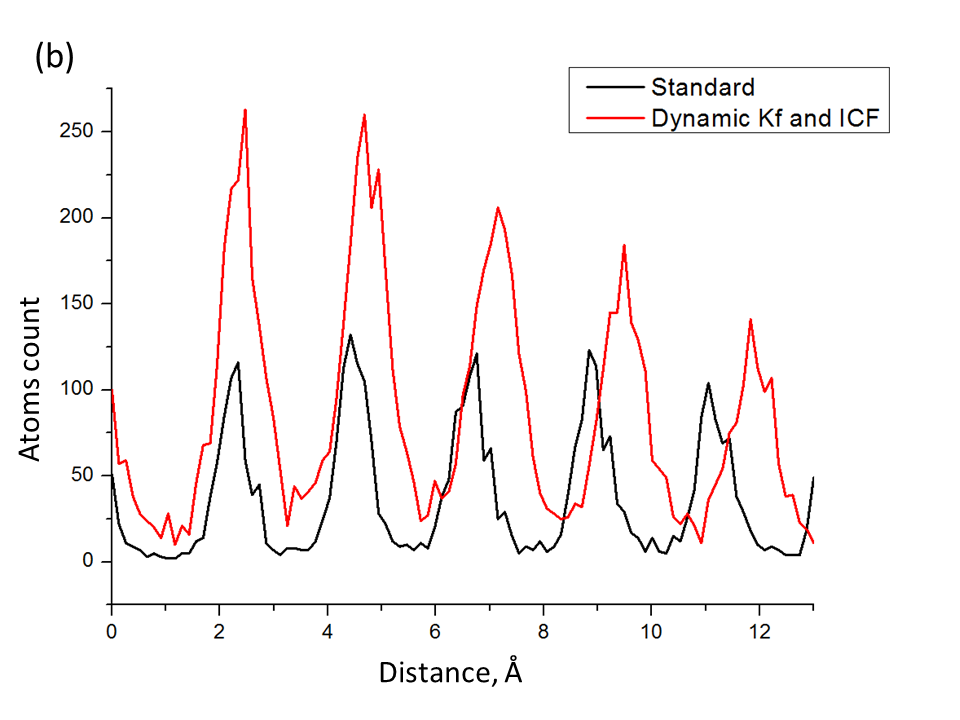
\includegraphics[width=\textwidth]{p3_atomiccount_distance}
	}
	\caption{Распределение расстояний между атомами \cite{scbibDensity}.}
	\label{fig:p3_atomiccount_distance}
\end{figure}


%\subsection{Подпараграф \cyrdash{} два}\label{subsec:ch3/sect33/sub2}

%Некоторый текст.

\FloatBarrier
\clearpage
\section{Основные результаты по главе 3}\label{sec:ch3/sect6}

В главе представлены результаты исследования вольфрама, которые подстверждают характеристики ПАЗЛ-3D в части пространственного разрешения и разрешения по массе. Проведен первичный подбор таких параметров исследования, как мощность лазерного излучения и поляризация пучка лазерного излучения. Обоснован выбор метрики контроля условий проведения исследований. В качестве основной такой метрики выбрано соотношение зарядностей основного химического элемента материала.

Определены зависимости параметров восстановления данных от испаряющего напряжения для образцов из алюминия и вольфрама. На основе полученных зависимостей предложен оригинальный протокол динамической реконструкции по плотности материал. Данная методика позволяет существенно сократить ошибку определения 3D координат атомов.










\clearpage
